\documentclass[11pt]{article}

\usepackage[a4paper,margin=20mm]{geometry}
\usepackage{graphicx}
\usepackage{amsmath}
\usepackage{booktabs}
\usepackage{colortbl}
\usepackage{tabularx}
\usepackage{algorithm}
\usepackage{algorithmic}
\usepackage[hidelinks]{hyperref}

\definecolor{TableHeader}{gray}{0.92}
\newcommand{\TableSetup}{%
  \footnotesize
  \setlength{\tabcolsep}{3pt}%
  \renewcommand{\arraystretch}{1.08}%
}
\renewcommand{\figurename}{Supplementary Figure}
\renewcommand{\tablename}{Supplementary Table}

\title{Supplementary Information for\\
Design and Audit of Resource-Constrained Predictive Multirobot Exploration}
\author{\parbox{0.95\textwidth}{\centering Haojia Gao, Haohua Que, Rongze Zhao, Qian Zhang, Mingkai Liu,
Jiajun Sun, Weihao Shan, Hoiian Au, Chunhong Yuan, Yusen Qin, Rong Zhao,
Lei Mu, Bokui Chen, Xueqian Wang, Qi Wei and Fei Qiao}}
\date{}

\begin{document}
\maketitle

\section*{Supplementary figures}

\begin{figure}[htbp]
  \centering
  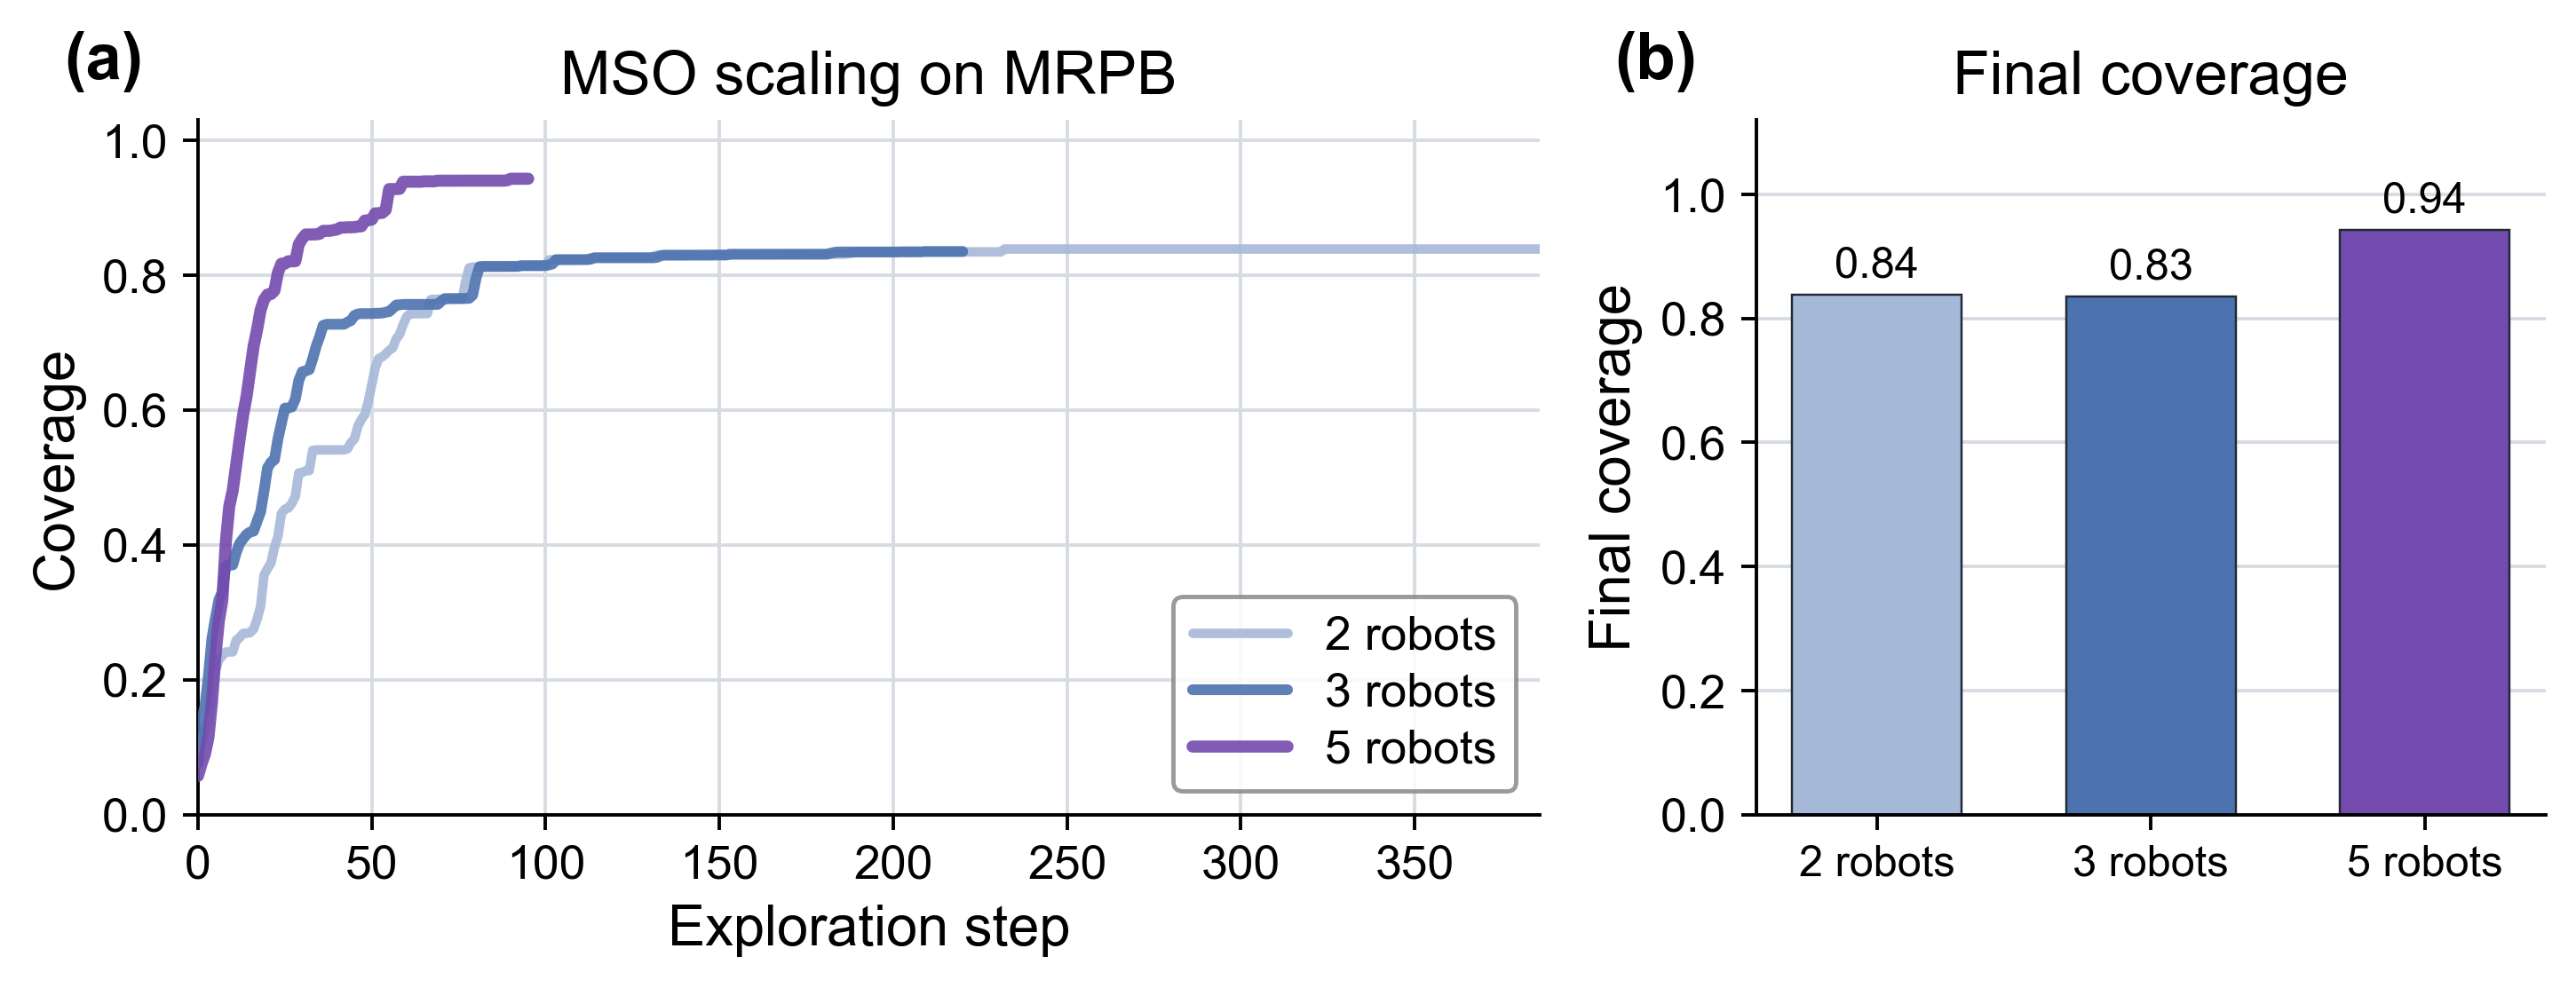
\includegraphics[width=0.94\textwidth]{supplementary_figure2.png}
  \caption{\textbf{Retained coverage traces from an auxiliary simulated team-size campaign.} \textbf{a}, One retained aggregate coverage trace for each $N\in\{2,3,5\}$ condition on its native logged-step axis. \textbf{b}, Coverage at the distinct recorded endpoint of each trace. The experiments were configured for five random seeds per condition, but run-level files and the campaign manifest were not retained; the plotted unit is therefore one aggregate trace per condition, not five independently displayed runs. The available files do not establish common initialisation, step definition, aggregation rule or software revision with the main 1500-step MRPB study. No seed-level variation or uncertainty interval can be reconstructed, and the curves are not interpreted as a controlled team-size effect or equal-horizon completion times. Machine-readable aggregate CSVs and the plotting script accompany the source-data archive.}
\end{figure}

\begin{figure}[htbp]
  \centering
  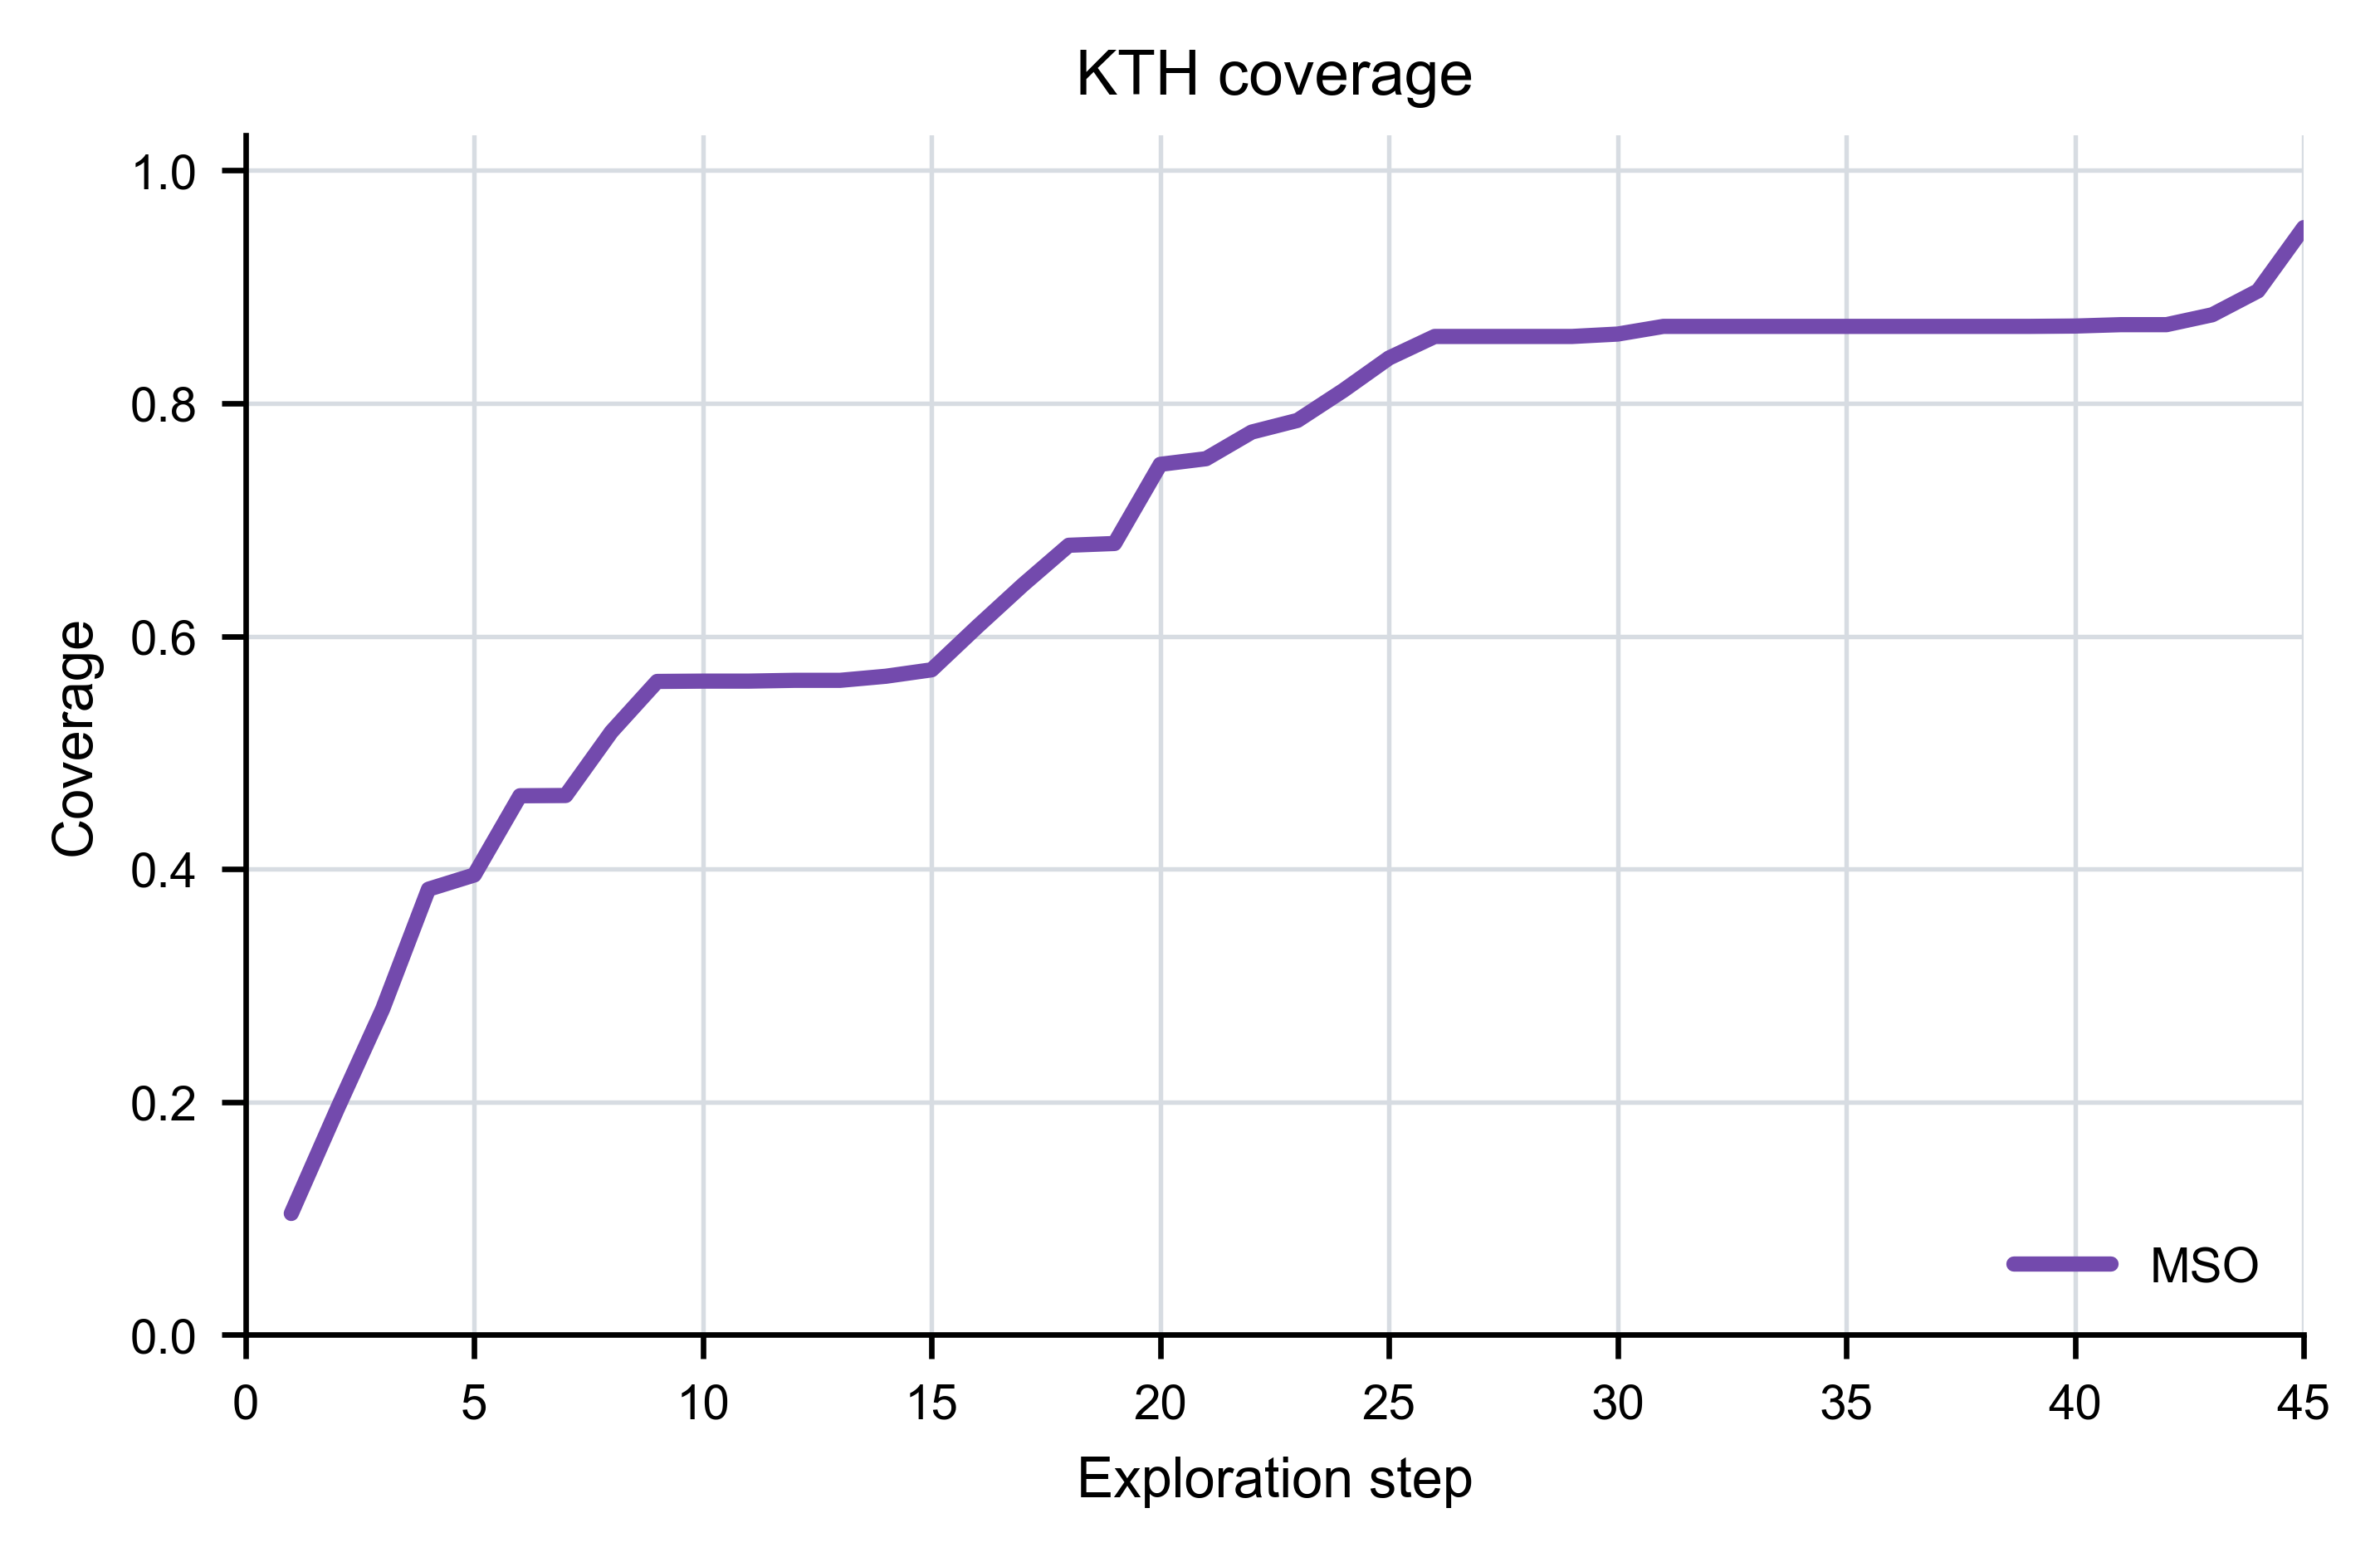
\includegraphics[width=0.68\textwidth]{supplementary_figure3.png}
  \caption{\textbf{Retained KTH coverage trace.} Full MSO on one KTH floorplan reported as held out. The panel shows all 45 rows of the retained aggregate coverage CSV without smoothing and ends at 0.950919. The experiment was configured for five random seeds, but run-level seed files were not retained, so the displayed unit is one aggregate trace and no seed-level variation or uncertainty interval is shown. The historical split manifest needed to verify the floorplan assignment was not recovered. The machine-readable coverage CSV and plotting script accompany the source-data archive. The unretained KTH occupied-cell-precision series is neither displayed nor analysed.}
\end{figure}

\begin{figure}[htbp]
  \centering
  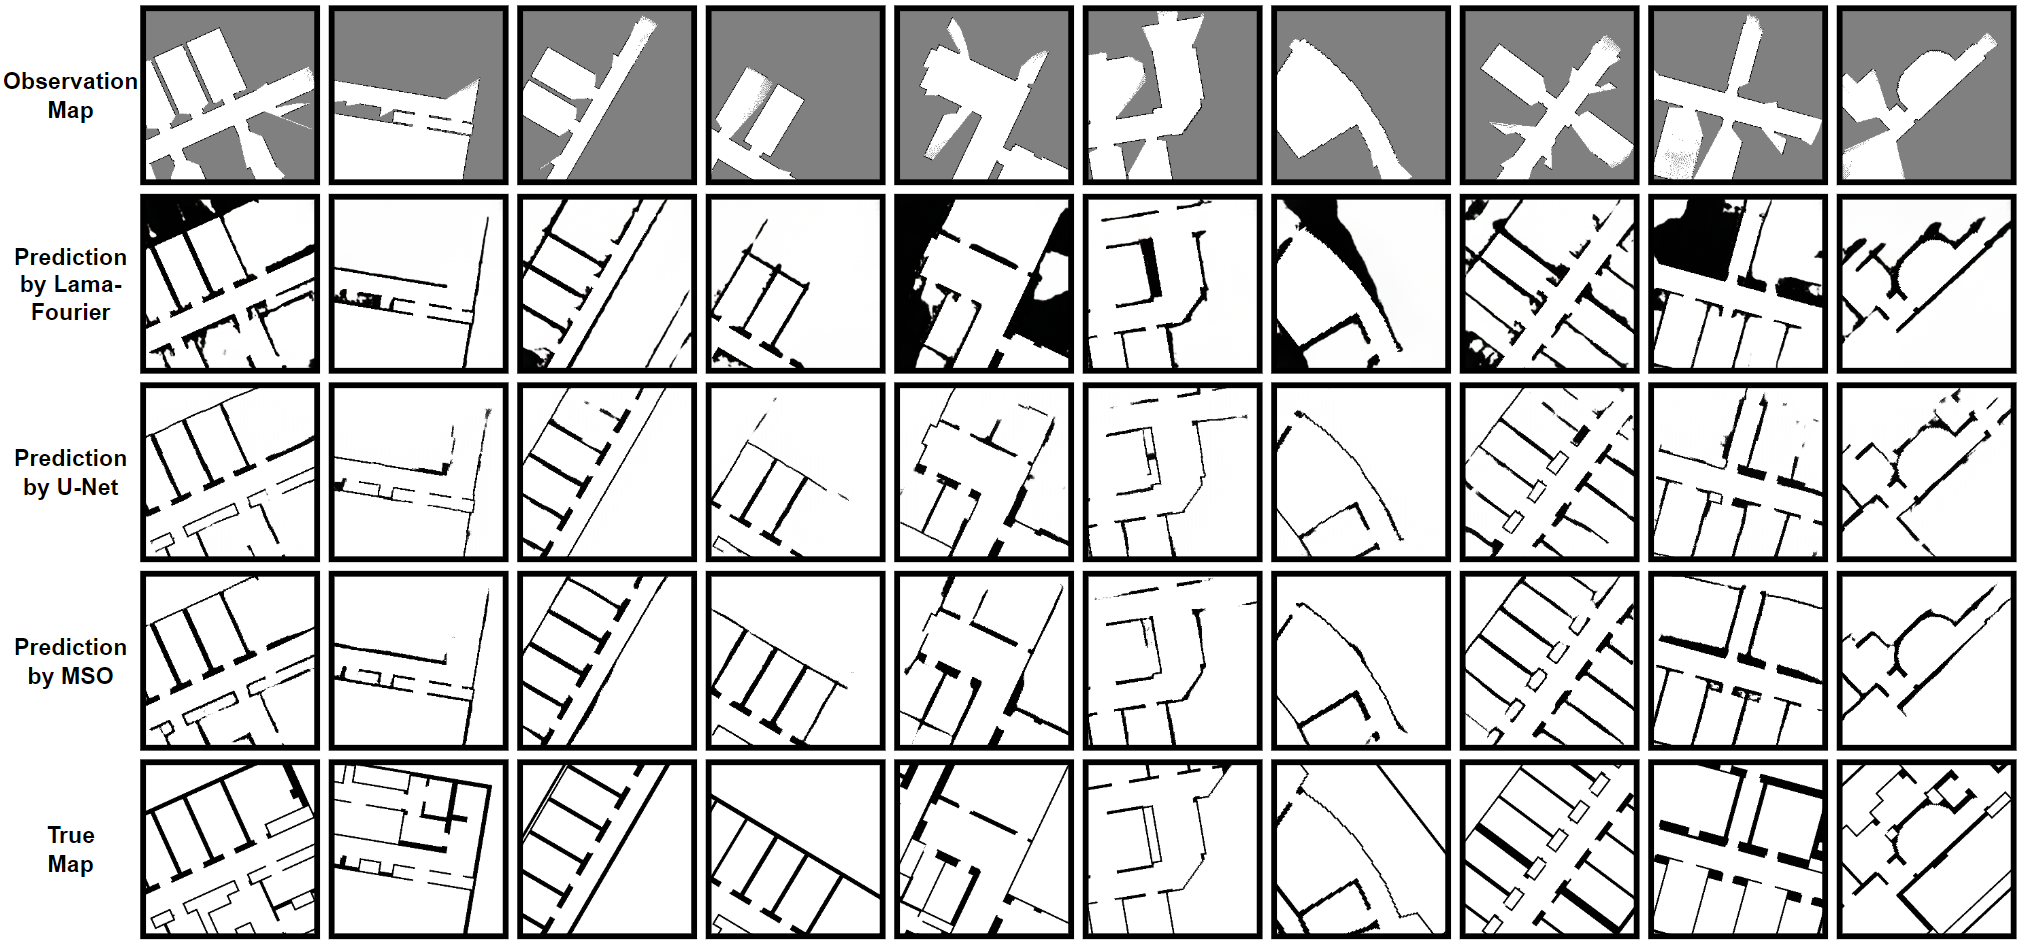
\includegraphics[width=\textwidth]{supplementary_figure4.png}
  \caption{\textbf{Additional local map-completion examples.} The display contains ten held-out evaluation crops ($n=10$ columns). Rows from top to bottom show the input observation, LaMa-Fourier prediction, U-Net prediction, MSO prediction and target map. These source images are qualitative examples and were not selected to estimate a population frequency of failure modes.}
\end{figure}

\begin{figure}[htbp]
  \centering
  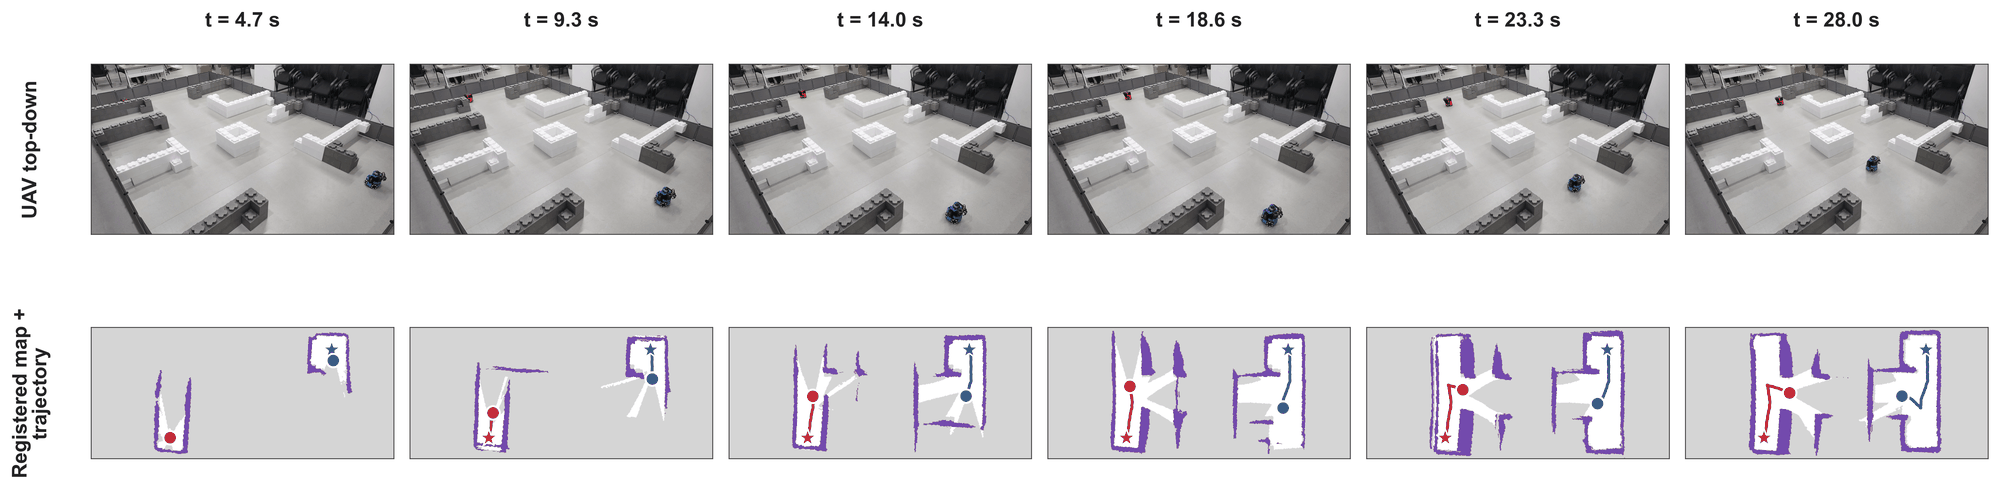
\includegraphics[width=\textwidth]{supplementary_dense_row1.png}\\[-0.35em]
  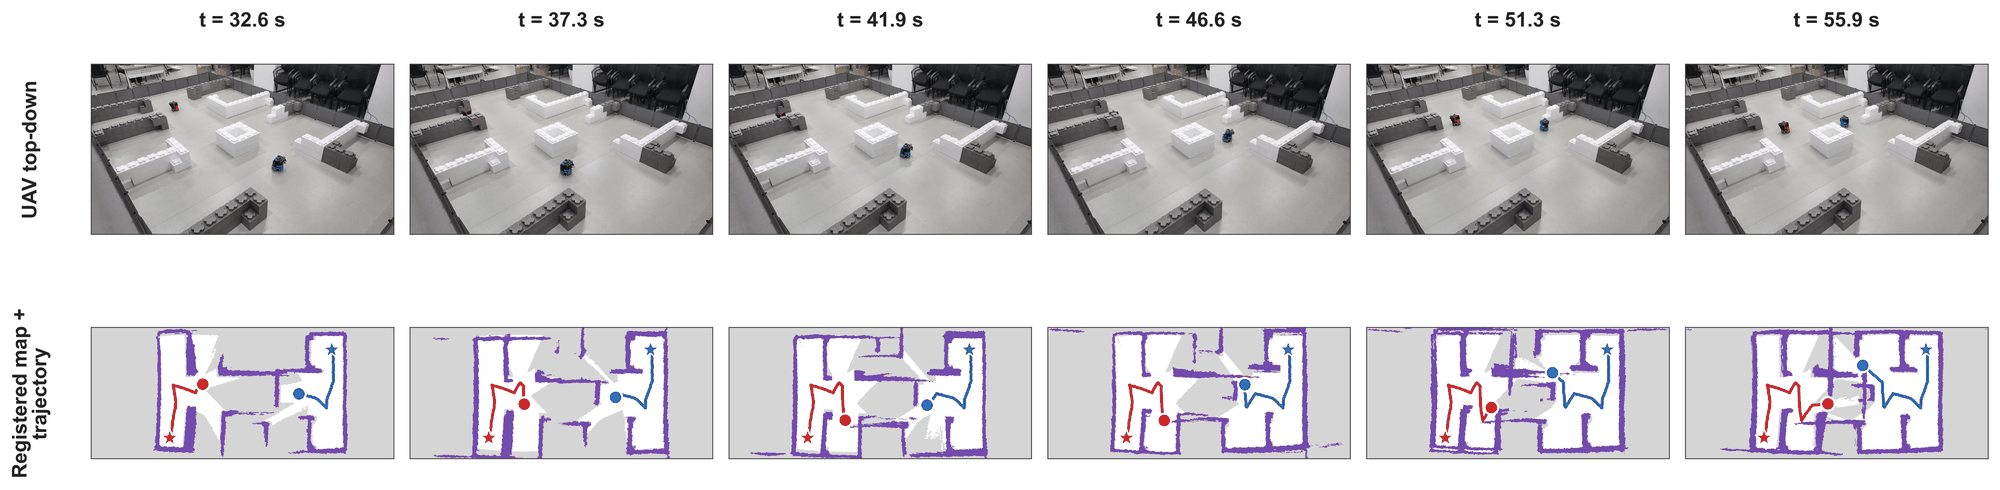
\includegraphics[width=\textwidth]{supplementary_dense_row2.png}\\[-0.35em]
  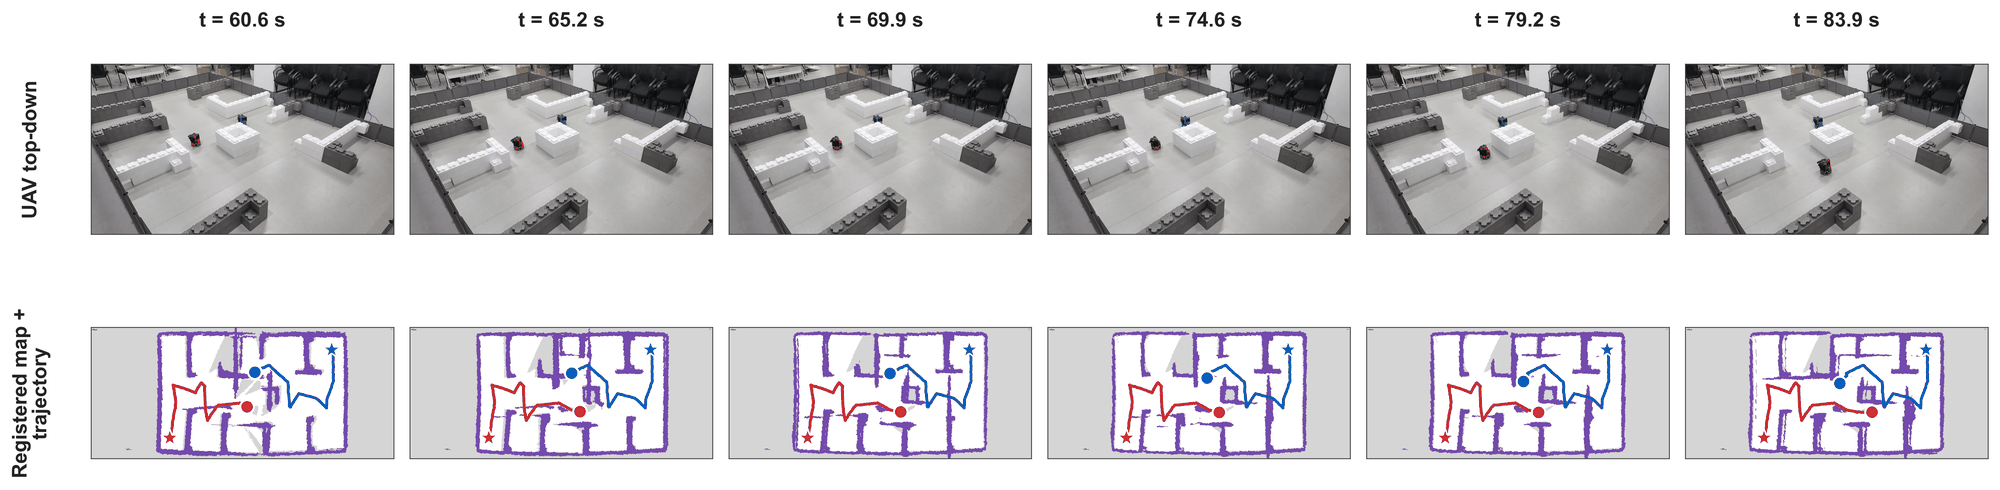
\includegraphics[width=\textwidth]{supplementary_dense_row3.png}\\[-0.35em]
  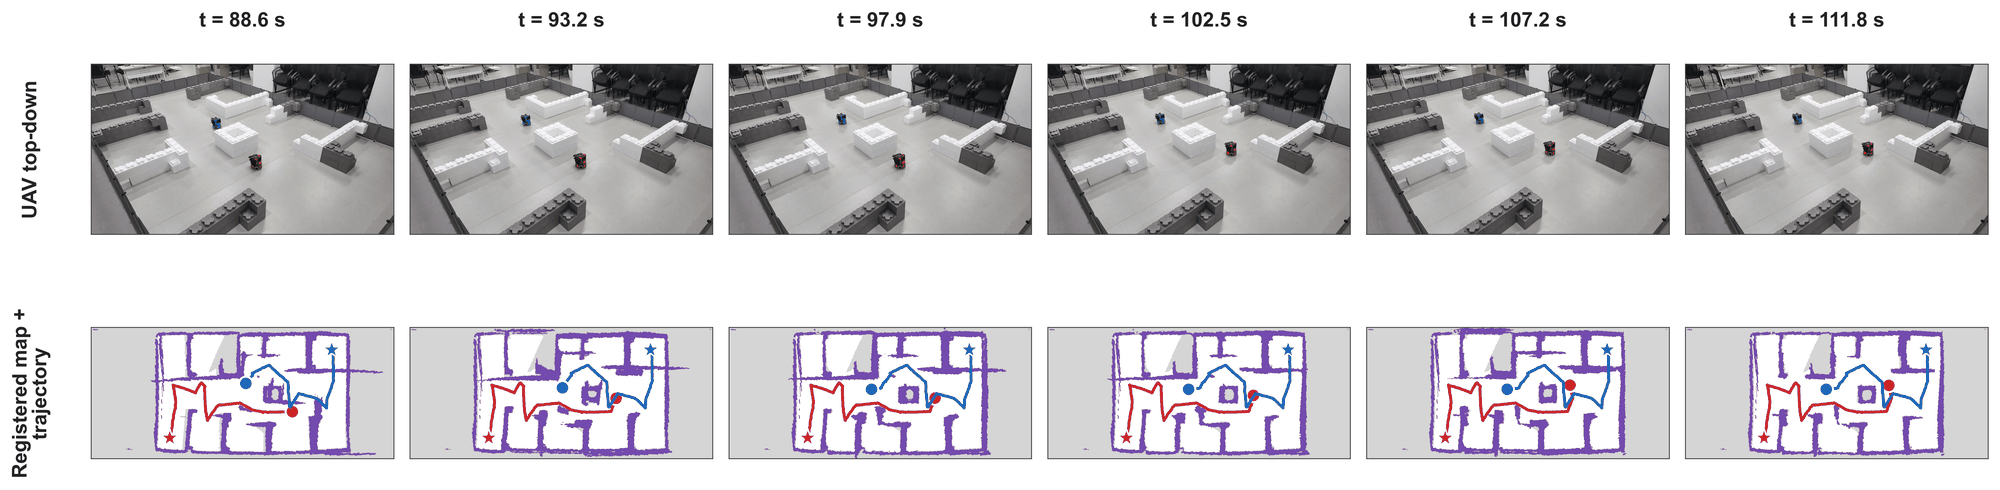
\includegraphics[width=\textwidth]{supplementary_dense_row4.png}
  \caption{\textbf{Dense progression of Scene 1.} Twenty-four equispaced snapshots from one MSO run ($n=1$ run; 24 displayed time points), ordered left-to-right and top-to-bottom. Each retained snapshot pairs an overhead image with an offline UAV-referenced map visualisation and robot trajectories. The sequence is a descriptive temporal display, not 24 independent replicates, and does not quantify transform drift, deployed registration accuracy or registration stability.}
\end{figure}

\begin{figure}[H]
  \centering
  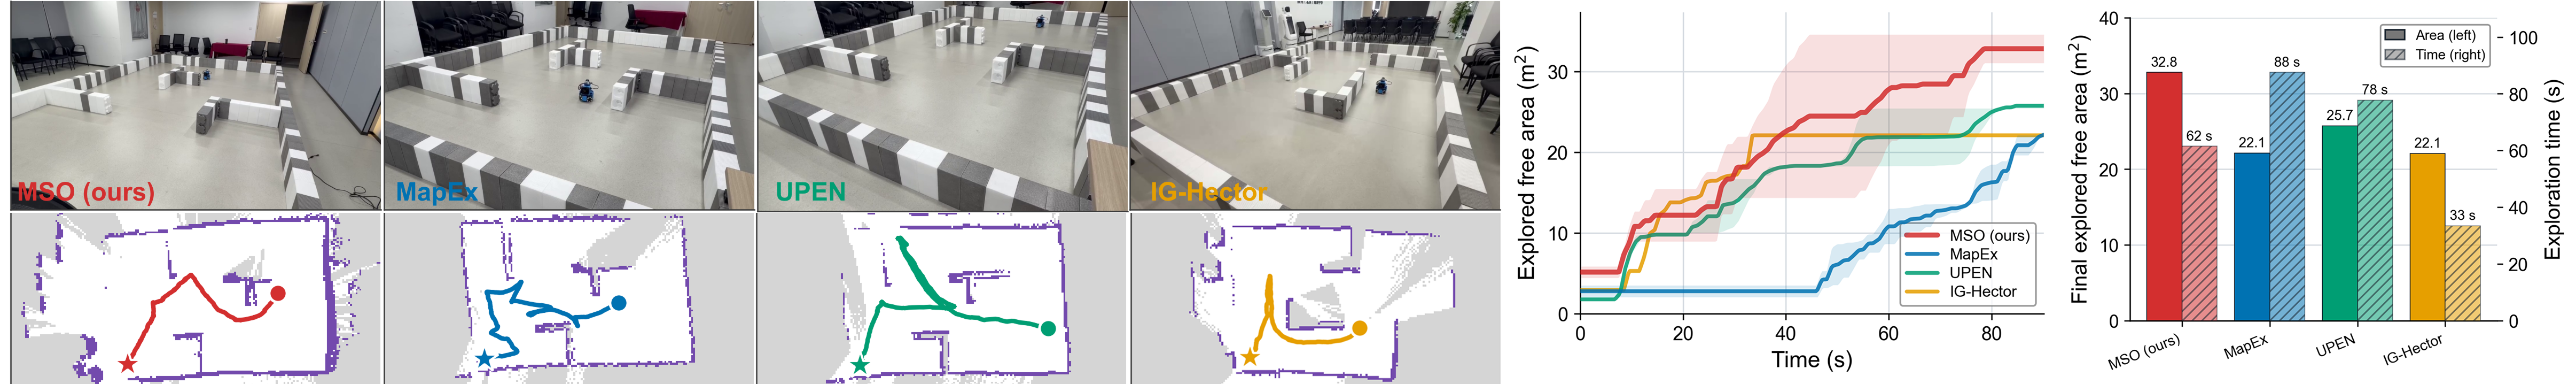
\includegraphics[width=\textwidth]{supplementary_single_robot.png}
  \caption{\textbf{Archived single-robot physical diagnostic.} Four planners were run on the same robot in one controlled arena. The photographs and maps show one representative retained run per method. The visible legacy ``explored free area'' label denotes the free-cell count over the complete unmasked \texttt{/map} raster multiplied by $(0.05\,\mathrm{m})^2$; it is not region-of-interest-clipped physical arena area or coverage. MSO, MapEx and UPEN each contribute two included successful runs, whereas IG-Hector contributes one because its 12.747-s failed first run was excluded from the plotted aggregate. Shading for the first three methods spans their two runs; IG-Hector has no run-level spread. Different planner stopping rules and unequal sample counts preclude matched-horizon or inferential comparison. All eight retained CSVs, including the excluded failed run, and the historical extraction script accompany the source-data archive.}
\end{figure}

\section*{Supplementary tables}

\begin{table}[H]
  \centering
  \caption{\textbf{Notation summary.}}
  \TableSetup
  \begin{tabularx}{\textwidth}{@{}>{\raggedright\arraybackslash}p{0.25\textwidth}>{\raggedright\arraybackslash}X@{}}
    \toprule
    \rowcolor{TableHeader}
    \textbf{Symbol} & \textbf{Meaning} \\
    \midrule
    $E$ & environment occupancy grid \\
    $M_i,\hat M_i$ & measured and predicted map maintained by robot $i$ \\
    $\widetilde O_t,O_E,P_{\mathrm{occ}}$ & reported occupied support, reference occupied support and occupied-cell precision \\
    $l,2l,4l$ & sensing, prediction and communication radii \\
    $x_{\mathrm{obs}},x_{\mathrm{true}},x_{\mathrm{pred}}$ & observation, target and predicted map \\
    $\sigma_p^2$ & deterministic Bernoulli ambiguity heuristic $\hat p(1-\hat p)$ \\
    $\mathcal{S},\mathcal{U}$ & Canny boundary-instability penalty and combined ambiguity score \\
    $w_m,\tau_w$ & match weight and match-weight threshold \\
    $\mathbf{H}_{\mathrm{space}}$ & candidate two-dimensional rigid transform \\
    $\Delta$ & occupancy-grid cell size \\
    \bottomrule
  \end{tabularx}
\end{table}

\begin{table}[htbp]
  \centering
  \caption{\textbf{Per-stage runtime on Jetson AGX Orin 32 GB in the 30 W profile.} LiDAR rasterisation runs every planner tick, MSO inference refreshes the prediction cache at approximately 1\,Hz, and the bottom group is event-driven.}
  \TableSetup
  \begin{tabularx}{\textwidth}{@{}>{\raggedright\arraybackslash}p{0.29\textwidth}>{\raggedright\arraybackslash}p{0.22\textwidth}>{\raggedright\arraybackslash}p{0.16\textwidth}>{\raggedright\arraybackslash}X@{}}
    \toprule
    \rowcolor{TableHeader}
    \textbf{Stage} & \textbf{Hardware unit} & \textbf{Latency} & \textbf{Notes} \\
    \midrule
    \multicolumn{4}{l}{\emph{Per-tick path}} \\
    LiDAR raster & 1$\times$ Cortex-A78AE & $\sim$2 ms & overlapped with the next sweep \\
    MSO inference and cache refresh & Ampere GPU & $\sim$3.0 ms & $\sim$1 Hz; TensorRT FP16, 342.8K parameters \\
    \midrule
    \multicolumn{4}{l}{\emph{Peer-encounter fusion path}} \\
    ORB extraction at three scales & 1$\times$ Cortex-A78AE & 12--18 ms & temporary leader \\
    Staged RANSAC and geometric filter & 1$\times$ Cortex-A78AE & 15--25 ms & up to 5000 iterations \\
    Overlap-aware blending & 1$\times$ Cortex-A78AE & 8--12 ms & overlap-dependent \\
    \textbf{Fusion event total} & & \textbf{40--60 ms} & per peer encounter \\
    \bottomrule
  \end{tabularx}
\end{table}

\begin{table}[htbp]
  \centering
  \caption{\textbf{ROS 2 topics exchanged between robots.} Payload is a typical size after the listed encoding.}
  \TableSetup
  \begin{tabularx}{\textwidth}{@{}>{\raggedright\arraybackslash}p{0.25\textwidth}>{\raggedright\arraybackslash}p{0.14\textwidth}>{\raggedright\arraybackslash}p{0.16\textwidth}>{\raggedright\arraybackslash}p{0.14\textwidth}>{\raggedright\arraybackslash}X@{}}
    \toprule
    \rowcolor{TableHeader}
    \textbf{Topic} & \textbf{Rate} & \textbf{Payload} & \textbf{Encoding} & \textbf{Contents} \\
    \midrule
    \texttt{/sensor/odom\_local} & 50 Hz & $\sim$80 B & native & pose and covariance \\
    \texttt{/mso/predicted\_map} & $\sim$1 Hz & 20--60 KB & run-length & predicted map and ambiguity score \\
    \texttt{/mso/feature\_packet} & event-driven & $<10$ KB & sparse & descriptors and match weights \\
    \bottomrule
  \end{tabularx}
\end{table}

\begin{table}[H]
  \centering
  \caption{\textbf{Empirical ROS 2 topic rates and serialised payloads from ten campaign rosbags.} Mean $\pm$ one sample standard deviation across bags or robot-topic streams. For per-robot topics, $n=20$ comprises two streams in each of ten bags and is not an independent-trial count. Values are uncompressed local ROS serialisation sizes.}
  \TableSetup
  \begin{tabular*}{\textwidth}{@{\extracolsep{\fill}}lcccc@{}}
    \toprule
    \rowcolor{TableHeader}
    \textbf{Topic} & \textbf{Samples} & \textbf{Rate (Hz)} & \textbf{Mean payload} & \textbf{Egress (KB/s)} \\
    \midrule
    \texttt{predicted\_map} (local) & 20 & $1.00\pm0.01$ & 278.6 KB & 277.7 \\
    \texttt{predicted\_map\_global} & 20 & $1.00\pm0.01$ & 417.7 KB & 416.2 \\
    \texttt{merged\_map} & 10 & $1.80\pm0.16$ & 335.9 KB & 601.4 \\
    \texttt{/robot\_X/map} & 20 & $0.31\pm0.03$ & 80.1 KB & 24.5 \\
    \texttt{/tf} & 10 & $19.22\pm0.27$ & 116 B & 2.2 \\
    \bottomrule
  \end{tabular*}
\end{table}

\begin{table}[htbp]
  \centering
  \caption{\textbf{Local map prediction comparison and ablation.} ``Operations'' reproduces the common profiler output in millions. The archived profiler output does not specify whether a multiply--accumulate is counted as one or two operations, so the values are used only for within-table comparison and are not labelled as FLOPs or MACs. All values are point estimates from one retained training run per method or variant.}
  \begingroup
  \setlength{\tabcolsep}{2.3pt}
  \renewcommand{\arraystretch}{1.06}
  \begin{tabularx}{\textwidth}{@{}>{\raggedright\arraybackslash}Xrrrrrrr@{}}
    \toprule
    \rowcolor{TableHeader}
    \textbf{Method} & \shortstack{\textbf{Params}\\$\downarrow$} & \shortstack{\textbf{Operations}\\$\downarrow$} & \shortstack{\textbf{PSNR}\\$\uparrow$} & \shortstack{\textbf{SSIM}\\$\uparrow$} & \shortstack{\textbf{LPIPS}\\$\downarrow$} & \shortstack{\textbf{FID}\\$\downarrow$} & \shortstack{\textbf{KID}\\$\downarrow$} \\
    \midrule
    U-Net & 31.040M & 54740.000 & 12.048 & 0.796 & 0.238 & 61.832 & 0.057 \\
    LaMa-Fourier & 27.000M & 66000.503 & 9.485 & 0.700 & 0.303 & 132.754 & 0.124 \\
    MI-GAN & 5.950M & 11024.197 & 10.067 & 0.637 & 0.403 & 274.933 & 0.307 \\
    MSO & 342.8K & 336.151 & 12.988 & 0.808 & 0.216 & 61.513 & 0.054 \\
    \midrule
    Full & 342.8K & 336.151 & 12.988 & 0.808 & 0.216 & 61.513 & 0.054 \\
    w/o adversarial & 342.8K & 336.151 & 12.955 & 0.808 & 0.216 & 68.915 & 0.061 \\
    w/o distillation & 342.8K & 336.151 & 12.951 & 0.810 & 0.216 & 74.313 & 0.068 \\
    w/o adversarial + distillation & 342.8K & 336.151 & 12.954 & 0.811 & 0.219 & 84.886 & 0.083 \\
    w/o FFC & 304K & 286.742 & 12.821 & 0.803 & 0.237 & 99.563 & 0.098 \\
    \bottomrule
  \end{tabularx}
  \endgroup
\end{table}

\begin{table}[H]
  \centering
  \caption{\textbf{Controlled offline relative-pose accuracy and selective reliability.} The archived reference implementation was reconstructed from the algorithm specification and was not replayed from the deployed executable. The selected one-scene test contains 50 known-transform positive encounters and 50 predeclared within-scene low-support abstention cases per input representation. Panel A includes every returned positive candidate before the gate; ``candidate/rigid'' gives all returned affines and the subset satisfying the near-unit SE(2) check. Errors are median [interquartile range] and P90. Panel B separates positive decisions from decisions on low-support cases, which have no unique pose-error label. Panel C bypasses feature matching and applies a fixed 1.0\,m and 15$^{\circ}$ error before a simulated atomic commit.}
  \begingroup
  \setlength{\tabcolsep}{2.3pt}
  \renewcommand{\arraystretch}{1.06}
  \begin{tabularx}{\textwidth}{@{}>{\raggedright\arraybackslash}Xrrrrrr@{}}
    \toprule
    \multicolumn{7}{l}{\textbf{Panel A: error on returned candidates from positive encounters}} \\
    \rowcolor{TableHeader}
    \textbf{Input} & \textbf{$n_{+}$} & \textbf{Cand./rigid} &
    \shortstack{\textbf{$e_t$ med.[IQR]}\\\textbf{(m)}} & \textbf{P90} &
    \shortstack{\textbf{$e_{\psi}$ med.[IQR]}\\\textbf{($^{\circ}$)}} & \textbf{P90} \\
    \midrule
    Observed & 50 & 50/50 & 0.040 [0.024, 0.061] & 0.072 & 0.023 [0.011, 0.040] & 0.080 \\
    Thresholded prediction & 50 & 50/45 & 0.052 [0.031, 0.079] & 0.143 & 0.052 [0.028, 0.118] & 0.193 \\
    Probability-preserving & 50 & 50/49 & 0.047 [0.029, 0.078] & 0.108 & 0.066 [0.023, 0.110] & 0.146 \\
    \bottomrule
  \end{tabularx}

  \vspace{0.4em}
  \begin{tabularx}{\textwidth}{@{}>{\raggedright\arraybackslash}Xrrrrrr@{}}
    \toprule
    \multicolumn{7}{l}{\textbf{Panel B: pre-commit decisions on positives and low-support cases}} \\
    \rowcolor{TableHeader}
    \textbf{Input} & \textbf{$n_{+}$} & \shortstack{\textbf{Correct}\\\textbf{accept}} &
    \shortstack{\textbf{Out-of-limit}\\\textbf{accept}} & \shortstack{\textbf{Positive}\\\textbf{reject}} &
    \shortstack{\textbf{Low-support}\\\textbf{A/R}} & \textbf{Total A/R} \\
    \midrule
    Observed & 50 & 50 & 0 & 0 & 0/50 & 50/50 \\
    Thresholded prediction & 50 & 43 & 0 & 7 & 9/41 & 52/48 \\
    Probability-preserving & 50 & 46 & 1 & 3 & 0/50 & 47/53 \\
    \bottomrule
  \end{tabularx}

  \vspace{0.4em}
  \begin{tabularx}{\textwidth}{@{}>{\raggedright\arraybackslash}Xrrrrr@{}}
    \toprule
    \multicolumn{6}{l}{\textbf{Panel C: wrong-transform injection and state-mutation audit}} \\
    \rowcolor{TableHeader}
    \textbf{Challenge} & \textbf{$n$} & \textbf{A/R} &
    \shortstack{\textbf{Reject before}\\\textbf{mutation}} & \shortstack{\textbf{Wrong}\\\textbf{commit}} &
    \shortstack{\textbf{Mutation after}\\\textbf{reject}} \\
    \midrule
    1.0\,m/15$^{\circ}$ error & 150 & 0/150 & 150/150 & 0/150 & 0/150 \\
    \bottomrule
  \end{tabularx}
  \endgroup
\end{table}

\begingroup
\footnotesize
\section*{Supplementary algorithm}
\vspace{-0.55em}

\begin{algorithm}[H]
  \caption{Predictive map-registration proposal}
  \begin{algorithmic}[1]
    \REQUIRE measured maps $\{M_i(t)\}$, provisional maps $\{\widehat M_i(t)\}$, probabilities $p_i$ and responses $S_i$
    \ENSURE a provisional transform, measured-support evidence and pre-commit decision
    \STATE form $U_i=\alpha p_i(1-p_i)+\beta S_i$, with $\alpha=0.7$ and $\beta=0.3$
    \STATE extract ORB, edge and morphology features at $1\times$, $0.5\times$ and $0.25\times$
    \STATE keep features with $U_i(k)<0.8\,\mathrm{mean}(U_i)$
    \STATE run KNN matching with Lowe ratio 0.9; use the retained direct-match fallback when fewer than eight matches remain
    \STATE retain matches with ambiguity weight $w_m>0.5$
    \STATE filter by displacement, scale and rotation consistency
    \STATE estimate a candidate with staged RANSAC thresholds $3.0/30\%$, $5.0/20\%$ and $10.0/3\%$
    \STATE refine $\widehat M_j\!\rightarrow\!\widehat M_i$ in the overlap and evaluate the gate only on measured support $M_i,M_j$
    \RETURN candidate, support evidence and decision; persistent state can change only through a separate, disabled-by-default atomic commit path after acceptance and temporal consensus
  \end{algorithmic}
\end{algorithm}
\enlargethispage{4\baselineskip}

\vspace{-0.45em}
\section*{Supplementary notes}
\vspace{-0.45em}

\subsection*{Supplementary Note 1: training-artifact provenance}
\vspace{-0.25em}
The historical experiment record reports 5{,}385 fitting crops, 1{,}356 held-out crops and 500 training epochs. It gives Adam $\beta_1=0.5$ and $\beta_2=0.999$. The exact sample-level split manifest, historical training entry, checkpoint-selection trace, several historical loss modules and manuscript checkpoint were not recovered. The closest preserved data archive contains 6{,}841 train-labelled and 1{,}463 test-labelled samples. These labels document the preserved directory structure and are not treated as a reconstruction of the manuscript split. A hash-verified inventory found no exact processed duplicate across the preserved labels, but the available identifiers do not support a reliable floorplan or building audit.

Two recovered generator-weight candidates strictly load into the reported 342{,}771-parameter student architecture. Both originate from epoch-499 checkpoints with global step 72{,}000, but neither is identified as the checkpoint used for Supplementary Table~5 or another manuscript result. Their embedded optimizer states use Adam betas $(0.0,0.99)$, which conflict with the historical setting reported above. The public reconstruction therefore preserves both records without resolving the difference by assumption. Its training and evaluation entry is a forward reconstruction; any values produced with it must be labelled reconstructed and kept separate from the historical point estimates.

\subsection*{Supplementary Note 2: offline replay of the deployment registrar}
\vspace{-0.25em}
The deployment-source audit is distinct from the controlled one-scene test in Supplementary Table~6. We replayed the recovered 2025 source on ten archived two-robot bags and exactly reproduced 1{,}325 of 1{,}485 recorded merged-map publications (89.2\%). The bags contain merged rasters but no transform or acceptance-decision topic. Exact raster equality therefore verifies many replayed outputs without recovering the transform or decision that produced each publication.

The legacy path estimates a partial affine and does not enforce a proper unit-scale two-dimensional rigid-body-group SE(2) constraint before publication. Among the 1{,}325 exactly reproduced publications, 1{,}263 associated candidates fail the near-unit SE(2) structural test and none passes structure together with the 0.25\,m and 5$^{\circ}$ diagnostic. We consequently tested a counterfactual proper-rigid estimator, a local gate and temporal consensus. Thresholds were fixed after inspecting \texttt{sense1-1}; the other nine bags were then held out from threshold development. Across 1{,}644 cached-map callbacks, the frozen audit produced eight counterfactual pre-commit acceptances after temporal consensus. None was within 0.25\,m and 5$^{\circ}$ of the UAV-derived reference, and two were within 0.50\,m and 10$^{\circ}$. Persistent-state commit remained disabled, yielding zero commits and 1{,}644 recommended rejections for this archive.

This is a negative offline audit. The gate and temporal-consensus manager were not deployed in the recorded bags, and the UAV-derived reference has non-negligible calibration residual. Cached-map callbacks are not independently labelled positive or negative encounters. The replay therefore does not estimate online transform accuracy, false-accept or false-reject rates, rollback success, contamination removal, or recovery time.

The conference draft contained a 200-clip streaming ablation of a temporal prior, but neither its clip manifest nor aggregate source record was recovered. It is therefore not reproduced as a numerical result in this submission.

\subsection*{Supplementary Note 3: physical team-size boundary}
\vspace{-0.25em}
All ten physical bags contain only robot~0 and robot~1; no simultaneous larger-team data were recovered. The $N\in\{2,3,5\}$ traces in Supplementary Fig.~1 are aggregates from a separate simulated campaign without its run manifest and do not establish scaling. Repository capture and audit protocols are future instrumentation, not evidence; physical scaling requires simultaneous, independently referenced, matched repetitions under a locked protocol.
\endgroup

\end{document}
